\chapter{Ejercicio: Domótica}
Para este ejercicio hay que simular el funcionamiento de una casa con sistemas de domótica.
Para su realización tengo cuatro archivos de \texttt{JavaScript} para cada una de las partes:
el servidor, el cliente, el agente y la página que simula los sensores.

El servidor será el que genera la base de datos, si existe antes la borra y la vuelve a crear, y
cuando cambien los sensores o el estado de los actuadores introducirá una nueva entrada en
la colección dedicada al historial. Además muestra por consola las nuevas conexiones que se
realicen por \texttt{socket.io}.

Para acceder a la página de los sensores tendremos que escribir \texttt{localhost:8080/sensores},
se nos mostrará un formulario para modificar los niveles de luminosidad y temperatura y más
abajo el estado de los actuadores: aire acondicionado, calefacción, persianas y luces.

\begin{figure}[!ht]
	\begin{center}
		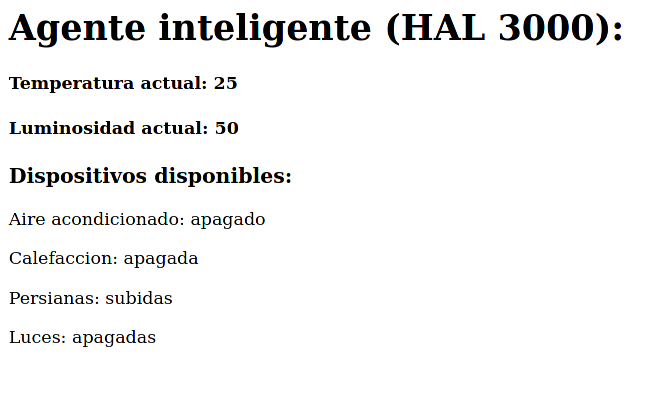
\includegraphics[scale=0.5]{sensores.png}
	\end{center}
\end{figure}

Para acceder a la página de los usuarios tendremos que escribir \texttt{localhost:8080/ciente},
esta página mostrará los niveles actuales de luminosidad y temperatura y nos permitirá cambiar
el estado de los actuadores. Si el agente modificase algo aparecería una alerta con qué ha
cambiado y por qué motivo.

\begin{figure}[!ht]
	\begin{center}
		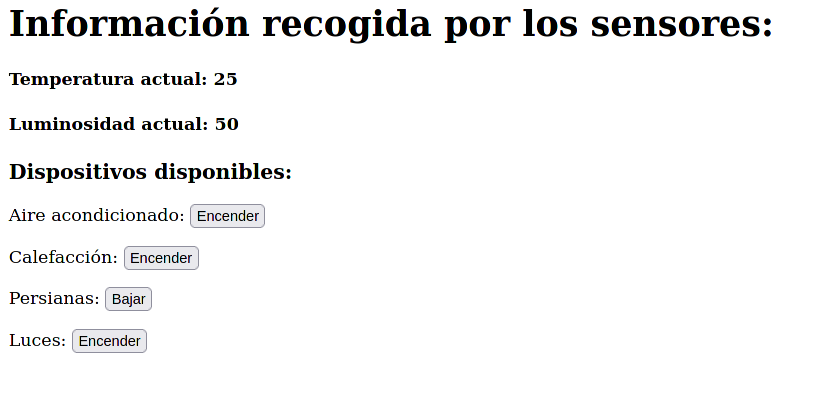
\includegraphics[scale=0.5]{cliente.png}
	\end{center}
\end{figure}

Para acceder a la página del agente tendremos que escribir \texttt{localhost:8080/agente},
mostrará los niveles actuales de luminosidad y temperatura y el estado de los actuadores.
Además activa o desactiva los actuadores según estas condiciones:
\begin{itemize}
	\item Si la temperatura es mayor que 30 y no esta activado el aire acondicionado lo enciende, cuando baja de 21 lo apaga.
	\item Si la temperatura es menor que 21 y la calefacción no está puesta la activa, cuando llega a 21 o más la apaga.
	\item Si el nivel de luminosidad es menor que 50 baja las persianas y enciende las luces.
\end{itemize}

\begin{figure}[!ht]
	\begin{center}
		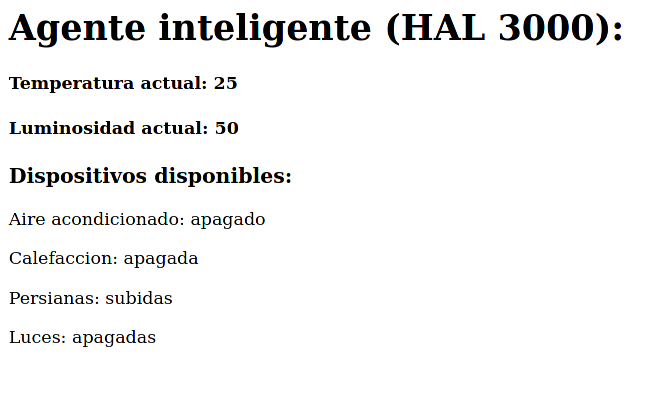
\includegraphics[scale=0.5]{sensores.png}
	\end{center}
\end{figure}
